\subsection{User-defined data types}
\label{subsec:library_of_transformations:type_level_transformations:user_defined_data_types}

\begin{figure}
    \centering
    \begin{subfigure}{0.45\textwidth}
        \centering
        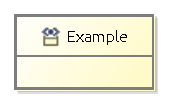
\includegraphics{images/05_library_of_transformations/02_type_level_transformations/05_user_defined_data_types/userdatatype_type.pdf}
        \caption{$Tm_{UserType}$ with $name = .\type{Example}$}
        \label{fig:library_of_transformations:type_level_transformations:user_defined_data_types:visualisation:ecore}
    \end{subfigure}
    \begin{subfigure}{0.45\textwidth}
        \centering
        % To use this figure in your LaTeX document
% import the package groove/resources/groove2tikz.sty
%
\begin{tikzpicture}[scale=\tikzscale,name prefix=test-]
\node[type_node] (n1) at (1.365, -0.595) {\ml{\textbf{Example}\\value: \textbf{string}}};

\end{tikzpicture}

        \caption{$TG_{UserType}$ with $name = .\type{Example}$\\ and $data\_\!edge = value$}
        \label{fig:library_of_transformations:type_level_transformations:user_defined_data_types:visualisation:groove}
    \end{subfigure}
    \caption{Visualisation of the transformation of user-defined data types}
    \label{fig:library_of_transformations:type_level_transformations:user_defined_data_types:visualisation}
\end{figure}

Within this section, the transformation of an user-defined data type will be defined. A user-defined data type in Ecore is a custom data type, of which a serialisation can be stored in the form of a string. The Ecore type model for introducing a user-defined data type is simple:

\begin{defin}[Type model $Tm_{UserType}$]
\label{defin:library_of_transformations:type_level_transformations:user_defined_data_types:tmod_userdatatype}
Let $Tm_{UserType}$ be the type model containing a user-defined data type with identifier $name$. $Tm_{UserType}$ is defined as:
\begin{align*}
Class =\ &\{\} \\
Enum =\ &\{\} \\
UserDataType =\ &\{name\} \\
Field =\ &\{\} \\
\mathrm{FieldSig} =\ &\{\} \\
EnumValue =\ &\{\} \\
Inh =\ &\{\} \\
Prop =\ &\{\} \\
Constant =\ &\{\} \\
\mathrm{ConstType} =\ &\{\}
\end{align*}
\isabellelref{tmod_userdatatype}{Ecore-GROOVE-Mapping-Library.UserDataTypeType}
\end{defin}

\begin{thm}[Correctness of $Tm_{UserType}$]
\label{defin:library_of_transformations:type_level_transformations:user_defined_data_types:tmod_userdatatype_correct}
$Tm_{UserType}$ (\cref{defin:library_of_transformations:type_level_transformations:user_defined_data_types:tmod_userdatatype}) is a consistent type model in the sense of \cref{defin:formalisations:ecore_formalisation:type_models:type_model_consistency}.
\isabellelref{tmod_userdatatype_correct}{Ecore-GROOVE-Mapping-Library.UserDataTypeType}
\end{thm}

A visual representation of $Tm_{UserType}$ with identifier $.\type{Example}$ can be seen in \cref{fig:library_of_transformations:type_level_transformations:user_defined_data_types:visualisation:ecore}. The correctness proof of $Tm_{UserType}$ is trivial, and therefore not included here. The proof can be found as part of the Isabelle validated proofs.

In order to make composing transformation functions possible, $Tm_{UserType}$ should be compatible with the type model it is combined with.

\begin{thm}[Correctness of $\mathrm{combine}(Tm, Tm_{UserType})$]
\label{defin:library_of_transformations:type_level_transformations:user_defined_data_types:tmod_userdatatype_combine_correct}
Assume a type model $Tm$ that is consistent in the sense of \cref{defin:formalisations:ecore_formalisation:type_models:type_model_consistency}. Then $Tm$ is compatible with $Tm_{UserType}$ (in the sense of \cref{defin:transformation_framework:type_models_and_type_graphs:combining_type_models:compatibility}) if:
\begin{itemize}
    \item The identifier of the user-defined data type in $Tm_{UserType}$ is not yet an identifier for a class, enumeration type or user-defined data type in $Tm$;
    \item The identifier of the user-defined data type in $Tm_{UserType}$ is not in the namespace of any class, enumeration type or user-defined data type in $Tm$;
    \item None of the identifiers in any class, enumeration type or user-defined data type in $Tm$ is in the namespace of the class in $Tm_{UserType}$.
\end{itemize}
\isabellelref{tmod_userdatatype_combine_correct}{Ecore-GROOVE-Mapping-Library.UserDataTypeType}
\end{thm}

\begin{proof}
Use \cref{defin:transformation_framework:type_models_and_type_graphs:combining_type_models:tmod_combine_merge_correct}. It is possible to show that all assumptions hold. Now we have shown that $\mathrm{combine}(Tm, Tm_{UserType})$ is consistent in the sense of \cref{defin:formalisations:ecore_formalisation:type_models:type_model_consistency}.
\end{proof}

The definitions and theorems for a regular class within Ecore are now complete. 

\subsubsection{Encoding as node type}

A possible encoding for user-defined data types in Ecore is using a node type in GROOVE. This node type will get a transformed identifier as name. In order to be able to store the serialised value, an edge type is created to a string node that represents the serialised value. The encoding corresponding to $Tm_{UserType}$ can then be represented as $TG_{UserType}$, defined in the following definition:

\begin{defin}[Type graph $TG_{UserType}$]
\label{defin:library_of_transformations:type_level_transformations:user_defined_data_types:tg_userdatatype_as_node_type}
Let $TG_{UserType}$ be the type graph containing a single node type which encodes a user-defined data type $name$. Furthermore, this node type has an edge type named $data\_\!edge$ to a string primitive to store its serialised value. $TG_{UserType}$ is defined as:
\begin{align*}
NT =\ &\{\mathrm{ns\_\!to\_\!list}(name)\} \\
ET =\ &\{(\mathrm{ns\_\!to\_\!list}(name), \langle data\_\!edge \rangle, \type{string})\} \\
\!\!\sqsubseteq\ =\ &\{( \mathrm{ns\_\!to\_\!list}(name), \mathrm{ns\_\!to\_\!list}(name) ), ( \type{string}, \type{string} )\} \\
abs =\ &\{\} \\
\mathrm{mult}(e) =\ &\begin{cases}
    (0..\mstar, 1..1) &\mathrm{if}\ e \in ET_{TG_{UserType}}
\end{cases}\\
contains =\ &\{\}
\end{align*}
\isabellelref{tg_userdatatype_as_node_type}{Ecore-GROOVE-Mapping-Library.UserDataTypeType}
\end{defin}

\begin{thm}[Correctness of $TG_{UserType}$]
\label{defin:library_of_transformations:type_level_transformations:user_defined_data_types:tg_userdatatype_as_node_type_correct}
$TG_{UserType}$ (\cref{defin:library_of_transformations:type_level_transformations:user_defined_data_types:tg_userdatatype_as_node_type}) is a valid type graph in the sense of \cref{defin:formalisations:groove_formalisation:type_graphs:type_graph_validity}.
\isabellelref{tg_userdatatype_as_node_type_correct}{Ecore-GROOVE-Mapping-Library.UserDataTypeType}
\end{thm}

A visual representation of $TG_{UserType}$ with identifier $.\type{Example}$ can be seen in \cref{fig:library_of_transformations:type_level_transformations:user_defined_data_types:visualisation:groove}. In this example, $value$ was chosen as edge name. The correctness proof of $TG_{UserType}$ is trivial, and therefore not included here. The proof can be found as part of the Isabelle validated proofs.

In order to make composing transformation functions possible, $TG_{UserType}$ should be compatible with the type graph it is combined with.

\begin{thm}[Correctness of $\mathrm{combine}(TG, TG_{UserType})$]
\label{defin:library_of_transformations:type_level_transformations:user_defined_data_types:tg_userdatatype_as_node_type_combine_correct}
Assume a type graph $TG$ that is valid in the sense of \cref{defin:formalisations:groove_formalisation:type_graphs:type_graph_validity}. Then $TG$ is compatible with $TG_{UserType}$ (in the sense of \cref{defin:transformation_framework:type_models_and_type_graphs:combining_type_graphs:compatibility}) if:
\begin{itemize}
    \item The node type of the encoded class in $TG_{UserType}$ is not a node type in $TG$.
\end{itemize}
\isabellelref{tg_userdatatype_as_node_type_combine_correct}{Ecore-GROOVE-Mapping-Library.UserDataTypeType}
\end{thm}

\begin{proof}
Use \cref{defin:transformation_framework:type_models_and_type_graphs:combining_type_graphs:tg_combine_merge_correct}. It is possible to show that all assumptions hold. Now we have shown that $\mathrm{combine}(TG, TG_{UserType})$ is valid in the sense of \cref{defin:formalisations:groove_formalisation:type_graphs:type_graph_validity}.
\end{proof}

The next definitions define the transformation function from $Tm_{UserType}$ to $TG_{UserType}$:

\begin{defin}[Transformation function $f_{UserType}$]
\label{defin:library_of_transformations:type_level_transformations:user_defined_data_types:tmod_userdatatype_to_tg_userdatatype_as_node_type}
The transformation function $f_{UserType}(Tm)$ is defined as:
\begin{align*}
NT =\ &\{\mathrm{ns\_\!to\_\!list}(u) \mid u \in UserDataType_{Tm}\} \cup \{\type{string}\} \\
ET =\ &\{(\mathrm{ns\_\!to\_\!list}(u), \langle data\_\!edge \rangle, \type{string}) \mid u \in UserDataType_{Tm}\}  \\
\!\!\sqsubseteq\ =\ &\{( \mathrm{ns\_\!to\_\!list}(u_1), \mathrm{ns\_\!to\_\!list}(u_2) ) \mid u_1 \in UserDataType_{Tm} \land u_2 \in UserDataType_{Tm} \}\ \cup\\& \{(\type{string}, \type{string})\} \\
abs =\ &\{\} \\
\mathrm{mult}(e) =\ &\begin{cases}
    (0..\mstar, 1..1) &\mathrm{if}\ e \in \{(\mathrm{ns\_\!to\_\!list}(u), \langle data\_edge \rangle, \type{string}) \mid u \in UserDataType_{Tm}\}
\end{cases}\\
contains =\ &\{\}
\end{align*}
\isabellelref{tmod_userdatatype_to_tg_userdatatype_as_node_type}{Ecore-GROOVE-Mapping-Library.UserDataTypeType}
\end{defin}

\begin{thm}[Correctness of $f_{UserType}$]
\label{defin:library_of_transformations:type_level_transformations:user_defined_data_types:tmod_userdatatype_to_tg_userdatatype_as_node_type_func}
$f_{UserType}(Tm)$ (\cref{defin:library_of_transformations:type_level_transformations:user_defined_data_types:tmod_userdatatype_to_tg_userdatatype_as_node_type}) is a valid transformation function in the sense of \cref{defin:transformation_framework:type_models_and_type_graphs:combining_transformation_functions:transformation_function_type_model_type_graph} transforming $Tm_{UserType}$ into $TG_{UserType}$.
\isabellelref{tmod_userdatatype_to_tg_userdatatype_as_node_type_func}{Ecore-GROOVE-Mapping-Library.UserDataTypeType}
\end{thm}

The proof of the correctness of $f_{UserType}$ will not be included here. Instead, it can be found in the validated Isabelle theories.

Finally, to complete the transformation, the transformation function that transforms $TG_{UserType}$ into $Tm_{UserType}$ is defined:

\begin{defin}[Transformation function $f'_{UserType}$]
\label{defin:library_of_transformations:type_level_transformations:user_defined_data_types:tg_userdatatype_as_node_type_to_tmod_userdatatype}
The transformation function $f'_{UserType}(TG)$ is defined as:
\begin{align*}
Class =\ &\{\} \\
Enum =\ &\{\} \\
UserDataType =\ &\{\mathrm{list\_\!to\_\!ns}(n) \mid n \in NT_{TG} \cap Lab_t \} \\
Field =\ &\{\} \\
\mathrm{FieldSig} =\ &\{\} \\
EnumValue =\ &\{\} \\
Inh =\ &\{\} \\
Prop =\ &\{\} \\
Constant =\ &\{\} \\
\mathrm{ConstType} =\ &\{\}
\end{align*}
\isabellelref{tg_userdatatype_as_node_type_to_tmod_userdatatype}{Ecore-GROOVE-Mapping-Library.UserDataTypeType}
\end{defin}

\begin{thm}[Correctness of $f'_{UserType}$]
\label{defin:library_of_transformations:type_level_transformations:user_defined_data_types:tg_userdatatype_as_node_type_to_tmod_userdatatype_func}
$f'_{UserType}(TG)$ (\cref{defin:library_of_transformations:type_level_transformations:user_defined_data_types:tg_userdatatype_as_node_type_to_tmod_userdatatype}) is a valid transformation function in the sense of \cref{defin:transformation_framework:type_models_and_type_graphs:combining_transformation_functions:transformation_function_type_graph_type_model} transforming $TG_{UserType}$ into $Tm_{UserType}$.
\isabellelref{tg_userdatatype_as_node_type_to_tmod_userdatatype_func}{Ecore-GROOVE-Mapping-Library.UserDataTypeType}
\end{thm}

Once more, the correctness proof is not included here but can be found in the validated Isabelle proofs of this thesis.